Conclusa la presentazione dell'approccio adottato nelle sperimentazioni, si procede in questo capitolo con l'esposizione dei risultati ottenuti. 

La macchina utilizzata nella risoluzione delle diverse istanze in questi esperimenti presenta le seguenti specifiche tecniche:
\begin{itemize}
\item
\item
\item
\end{itemize}

\newpage
\section{Risultati per grafi $G(n,p)$}
La prima categoria di grafi di cui sono stati analizzati i risultati sono i grafi $G(n,p)$, generati utilizzando il modello di Erdős–Rényi. 

Per prima cosa è stata studiata la correlazione tra la probabilità di generazione di ogni arco $p$ e il tempo impiegato dal risolutore nella soluzione dell'istanza del problema di vertex cover $time$, per ciascuno dei parametri di dimensione utilizzati. Per fare questo è stato disegnato un grafico, riportato di seguito in Figura \ref{fig:gnp2d}.
\begin{figure}[h!]
     \centering
       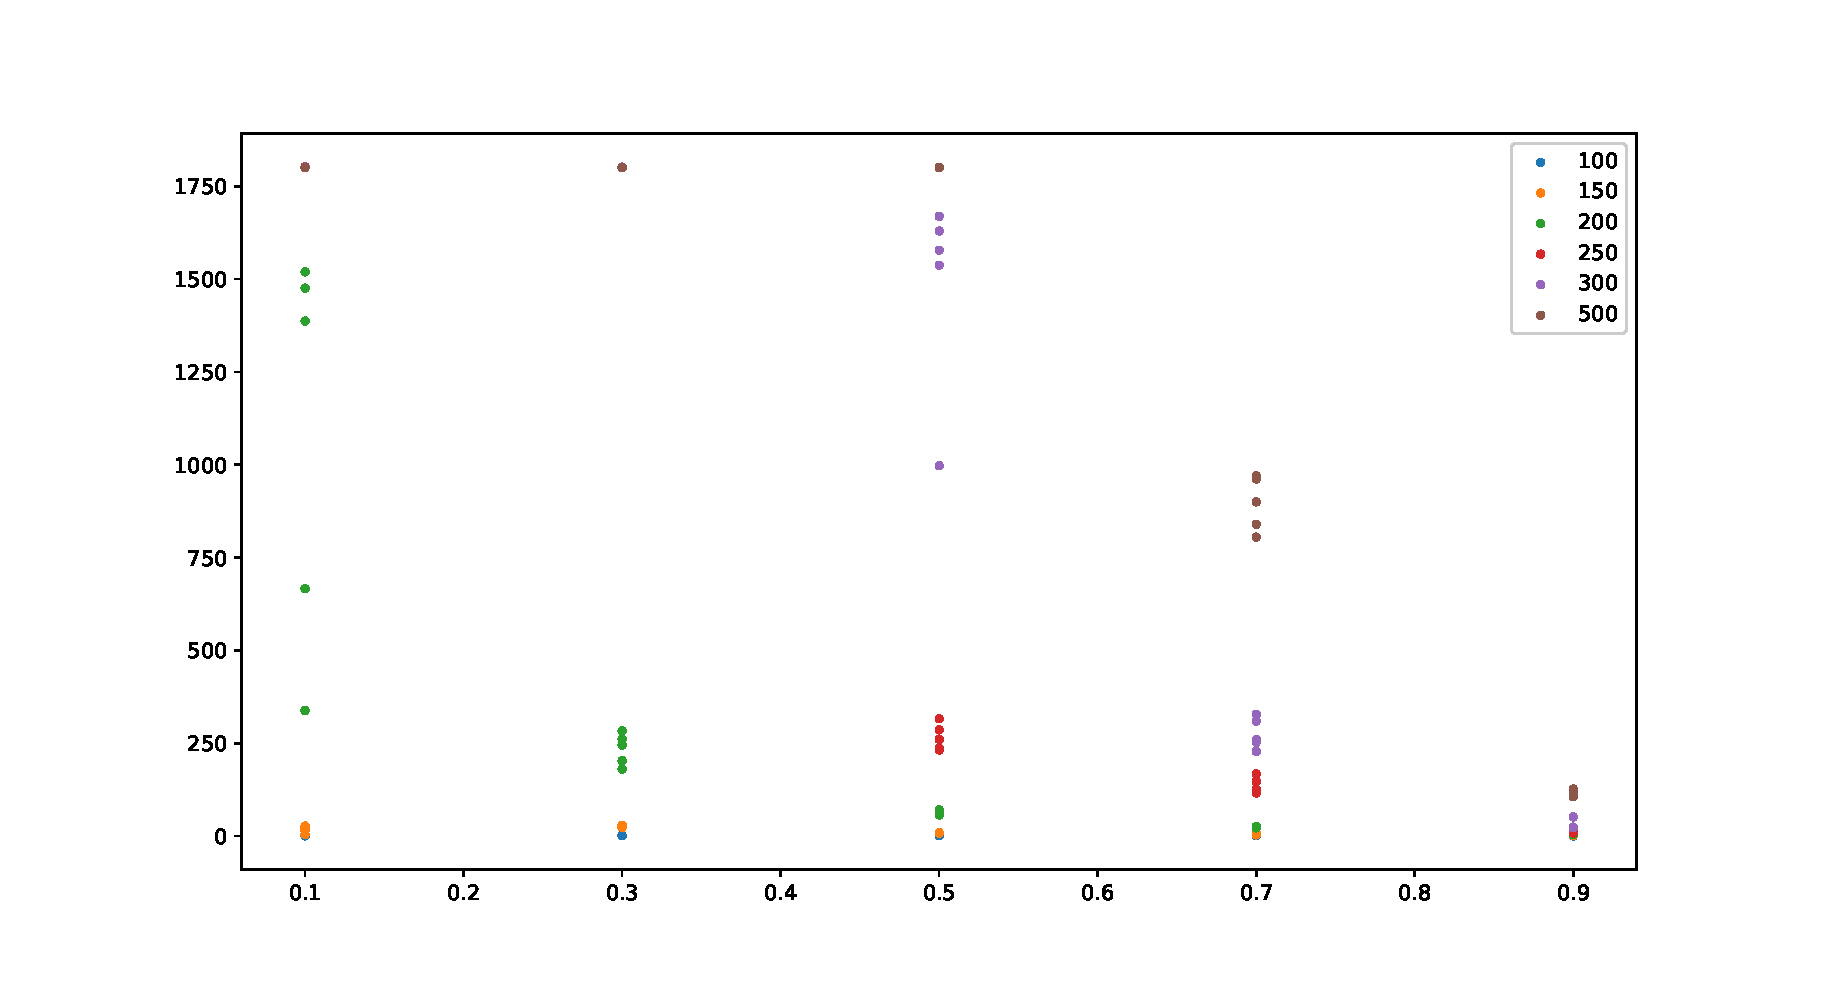
\includegraphics[scale=0.4]{images/gnp-2d.eps}
       \caption{Correlazione tra tempo di risoluzione $time$ (ordinata) e probabilità di generazione di ciascun arco $p$ (ascissa).}
        \label{fig:gnp2d}
\end{figure}

Oltre al semplice plot dei dati, in questo grafico è stata estrapolata una curva da ciascuno degli insiemi di misurazioni di ogni dimensione (applicando la regressione lineare), in modo tale da riuscire ad approssimarne l'andamento. Il grafico risultante evidenzia una chiara relazione di tipo esponenziale inverso tra $p$ e $time$. Istanze 

Anche la dimensione dell'istanza di grafo sembra giocare un ruolo relativamente importante nella determinazione della complessità del problema di vertex cover associato, essendo apparentemente responsabile per la velocità con cui l'esponenziale satura.
Per approfondire meglio il ruolo della dimensione nella determinazione della complessità di risoluzione, sono stati 

\begin{figure}[h!]
     \centering
       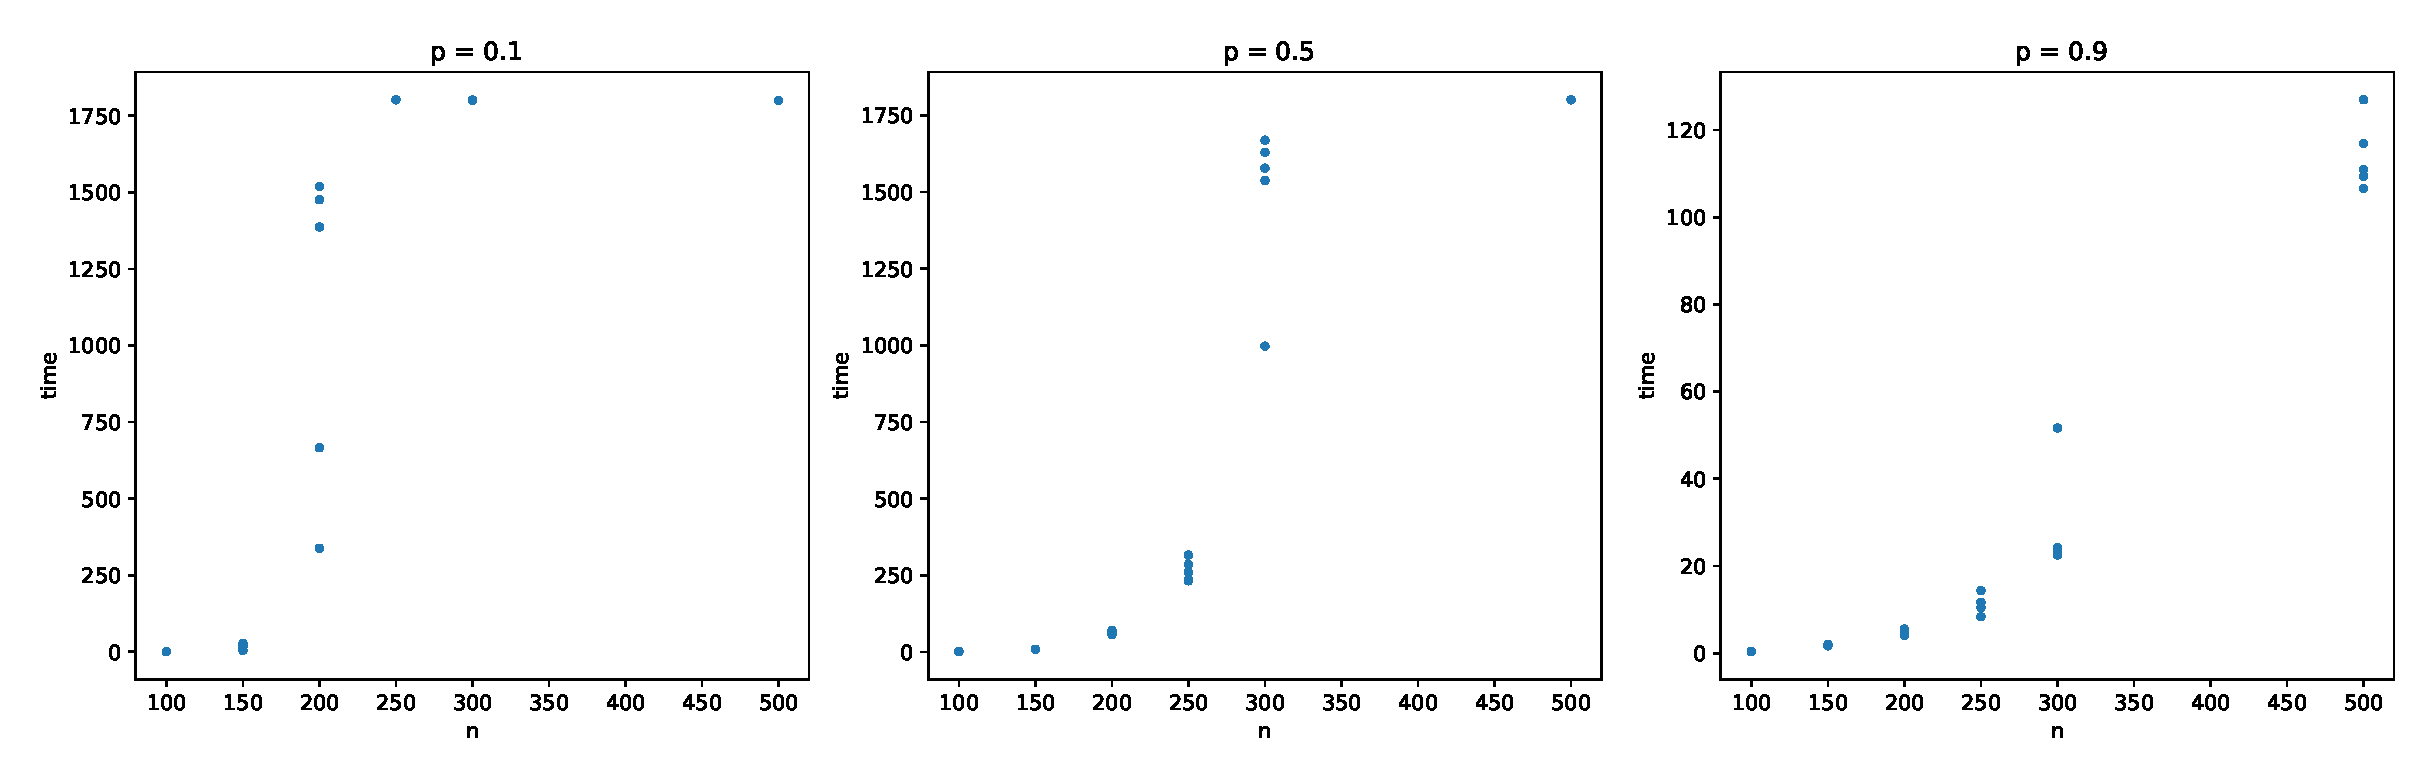
\includegraphics[scale=0.4]{images/gnp_p.eps}
       \caption{Correlazione tra tempo di risoluzione $time$ (ordinata) e probabilità di generazione di ciascun arco $p$ (ascissa).}
        \label{fig:gnp2d}
\end{figure}

\begin{figure}[h!]
     \centering
       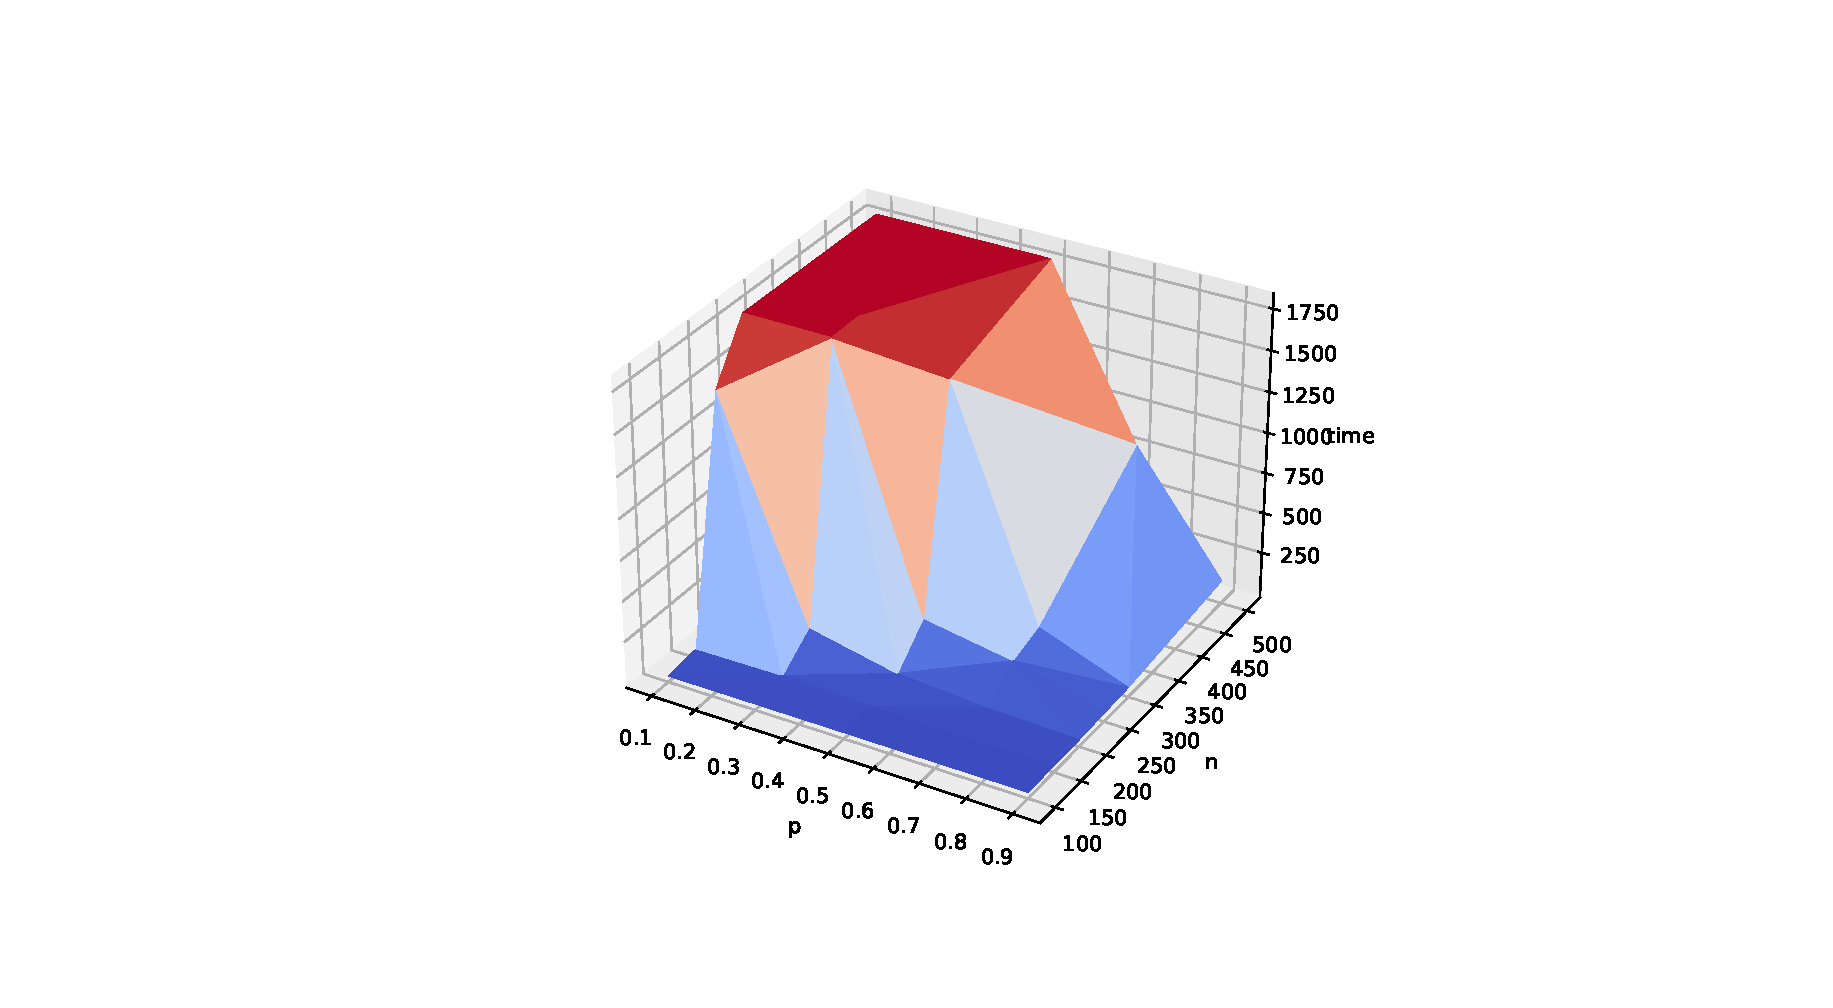
\includegraphics[scale=0.4]{images/gnp-3d.eps}
       \caption{Correlazione tra tempo di risoluzione $time$ (ordinata) e probabilità di generazione di ciascun arco $p$ (ascissa).}
        \label{fig:gnp2d}
\end{figure}

\section{Grafi regolari}

\section{Grafi di Watts-Strogatz}

\section{Grafi di Barabási-Albert}